% USEFUL LINKS:
% -------------
%
% - UiO LaTeX guides:          https://www.mn.uio.no/ifi/tjenester/it/hjelp/latex/
% - Mathematics:               https://en.wikibooks.org/wiki/LaTeX/Mathematics
% - Physics:                   https://ctan.uib.no/macros/latex/contrib/physics/physics.pdf
% - Basics of Tikz:            https://en.wikibooks.org/wiki/LaTeX/PGF/Tikz
% - All the colors!            https://en.wikibooks.org/wiki/LaTeX/Colors
% - How to make tables:        https://en.wikibooks.org/wiki/LaTeX/Tables
% - Code listing styles:       https://en.wikibooks.org/wiki/LaTeX/Source_Code_Listings
% - \includegraphics           https://en.wikibooks.org/wiki/LaTeX/Importing_Graphics
% - Learn more about figures:  https://en.wikibooks.org/wiki/LaTeX/Floats,_Figures_and_Captions
% - Automagic bibliography:    https://en.wikibooks.org/wiki/LaTeX/Bibliography_Management  (this one is kinda difficult the first time)
%
%                              (This document is of class "revtex4-1", the REVTeX Guide explains how the class works)
%   REVTeX Guide:              http://www.physics.csbsju.edu/370/papers/Journal_Style_Manuals/auguide4-1.pdf
%
%
% COMPILING THE .pdf FILE IN THE LINUX TERMINAL
% ---------------------------------------------
%
% [terminal]$ pdflatex report_example.tex
%
% Run the command twice, always.
%
% When using references, footnotes, etc. you should run the following chain of commands:
%
% [terminal]$ pdflatex report_example.tex
% [terminal]$ bibtex report_example
% [terminal]$ pdflatex report_example.tex
% [terminal]$ pdflatex report_example.tex
%
% This series of commands can of course be gathered into a single-line command:
% [terminal]$ pdflatex report_example.tex && bibtex report_example.aux && pdflatex report_example.tex && pdflatex report_example.tex
%
% ----------------------------------------------------



% \documentclass[english,notitlepage,reprint,nofootinbib]{revtex4-2}  % defines the basic parameters of the document
% \documentclass[english,notitlepage,reprint,nofootinbib]{revtex4-2}  % defines the basic parameters of the document
% \documentclass[english,notitlepage,reprint]{revtex4-2}  % defines the basic parameters of the document
% \documentclass[aps,prl,reprint,amsmath,amssymb,twocolumn,preprintnumbers,superscriptaddress,10pt]{revtex4-2}
\documentclass[aps,pra,reprint,amsmath,amssymb,twocolumn,preprintnumbers,superscriptaddress,10pt]{revtex4-2}
% If you want a single-column, remove "reprint"
% \raggedbottom


% Allows special characters (including æøå)
\usepackage[utf8]{inputenc}
% \usepackage[english]{babel}

% Note that you may need to download some of these packages manually, it depends on your setup.
% It may be usefult to download TeXMaker, because it includes a large library of the most common packages.


%%%%%%%%%%% Important packages %%%%%%%%%%%
\usepackage{coffeestains}
% \AddToHookNext{shipout/background}{%
%   \coffeestainA{0.8}{1}{-25}{5cm}{1.5cm}%
% }

% \AddToHookNext{shipout/background}{%
%   \coffeestainC{1}{1}{180}{0}{-5mm}%
% }

% \directlua{package.path = package.path .. ";./?.lua;./?/init.lua"}
% \usepackage{typewriter}
% \providecommand\ttgreybolda{0.6}
% \providecommand\ttgreyboldb{0.3}
% \providecommand\ttrotatebold{12}
% \providecommand\ttdownbold{20000}
% \providecommand\ttrightbold{35000}
% \providecommand\ttoverprintbolda{1}
% \providecommand\ttoverprintboldb{1}
% \providecommand\ttoverprintboldc{1}
% \providecommand\ttgreynormala{0.3}
% \providecommand\ttgreynormalb{0.5}
% \providecommand\ttrotatenormal{8}
% \providecommand\ttrightnormal{20000}
% \providecommand\ttdownnormal{20000}
% \providecommand\ttoverprintnormal{1}
% \providecommand\ttbasefont{cmuntt.otf}
% \providecommand\ttmathfont{\ttbasefont}
% \providecommand\ttfontsize{12pt}

%%%%%%%%%%% Important packages %%%%%%%%%%%
% \usepackage[justification=raggedright,singlelinecheck=false]{caption}
\usepackage{physics,amssymb}   % physics already loads amsmath
% \usepackage{amsmath}         
\usepackage{graphicx}
\usepackage{siunitx}
\usepackage{xcolor}
\usepackage{listings}
% \usepackage{subcaption}
% \usepackage{subfig}
\usepackage[caption=false]{subfig}
\usepackage{standalone}   % for \includestandalone
\usepackage{algorithm}
\usepackage[noend]{algpseudocode}
\definecolor{codegreen}{RGB}{87,166,74}
\algrenewcommand\algorithmiccomment[1]{\hfill\textcolor{codegreen}{\textit{// #1}}}
\newcommand{\AlgComment}[1]{\Statex \textcolor{codegreen}{\textit{// #1}}}

% \algrenewcommand\algorithmiccomment[1]{\hfill\textcolor{green}{// #1}}

\usepackage[acronym]{glossaries}    % e.g. partial density function (pdf)
\makeglossaries

% Acronyms:
\newacronym{pdf}{PDF}{partial density function}
\newacronym{mcmc}{MCMC}{Markov chain Monte Carlo}
\newacronym{wlln}{WLLN}{Weak Law Of Large Numbers}
\newacronym{lln}{LLN}{Law Of Large Numbers}
\newacronym{mcse}{MCSE}{Monte Carlo standard error}
\newacronym{ess}{ESS}{effective sample size}


\usepackage{tikz}
\usepackage{quantikz}          
\usepackage{hyperref}
\usepackage{float}             % optional, for [H] placement


\hypersetup{
    colorlinks,
    linkcolor={red!50!black},
    citecolor={blue!50!black},
    urlcolor={blue!80!black}
}


% ===================== Shortcuts/new commands ======================
\renewcommand{\vec}[1]{\mathbf{#1}}

\newcommand{\eqdef}{\mathrel{\mathop:}=}
\newcommand{\eqdefback}{\mathrel{=\mathop:}}

\begin{document}

\title{PROJECT 5 NAME\\[0.5em]
  \small \href{https://github.uio.no/icrukan/FYS4150/tree/master/Project5}{\texttt{github.uio.no/icrukan/FYS4150/Project5}}
}
\author{Magnus Axelsen and Isak Cecil Onsager Rukan} % self-explanatory
\date{\today}                             % self-explanatory
\noaffiliation                            % ignore this, but keep it.

\begin{abstract}
    Abstract
\end{abstract}
\maketitle

\section{Introduction}
The double slit experiment is a famous demonstration of the wave-properties of matter and light in quantum mechanics.

The double slit experiment was first conducted by Thomas Young in 1801 \cite{Young1804}.

\section{Theory and Method} \label{sec:theory_and_method}

\subsection{Quantum Mechanics and the double slit}

The evolution of a quantum system is famously described by the Schr\"{o}dinger equation, whose general form is given by
\begin{align}
    i \hbar \dv{}{t}\ket{\Psi} = \hat{H} \ket{\Psi},
\end{align}
where $\ket{\Psi}$ is the quantum state, $\hat{H}$ is the Hamiltonian operator, and $\hbar$ is the reduced Planck constant. The wave function \(\Psi(\vec{x}; t)\) is given by the projection of \(\ket{\Psi}\) onto the position eigenbasis:
\begin{align}
    \Psi(\vec{x}; t) = \bra{\vec{x}}\ket{\Psi}.
\end{align}
Letting \(\ket{\Psi}\) represent a single particle state, the wave function encodes the probability of detecting this particle at some position in time.
More precisely, the probability density \(p(\vec{x};t)\) for detecting a particle at position \(\vec{x}\) is given by
\begin{align}
    p(\vec{x};t) = |\Psi(\vec{x},t)|^2.    \label{eq:Born_rule}
\end{align}
This is a special case of the Born rule~\footnote{For an introduction to the Born rule or related concepts, see any standard quantum-mechanics textbook, such as \cite{GriffithsSchroeter2018}.}.

Here, we will be interested in the case of a single non-relativistic particle in two dimensions, propagating towards a barrier with a single, double or triple slit.
We denote the single particle's wave function as \(u(x,y,t)\).
Simplified to its dimensionless form, the Schr\"{o}dinger equation is then given by
\begin{align} \label{eq:schrodinger_equation}
   i \pdv{u}{t} = -\nabla^2 u + v(x,y) u,
\end{align}
where $u = u(x,y,t)$ is the wave function, $v(x,y)$ is a given potential, and $\nabla^2 = \pdv[2]{}{x} + \pdv[2]{}{y}$ is the Laplace operator in two dimensions.

Modelling a slit experiment, we let the potential \(v(x,y)\) be zero everywhere aside from the barrier, where we assign it some constant value $v_0$, which we refer to as the \emph{barrier height}.
The potential will in principle be material specific, and determines the reflection and transmission coefficients of the barrier.
We imagine the barrier as strongly reflecting and will set \(v_0\) to be large value in our simulation.

\subsection{Setup and initial state}
Working with the dimensionless version of the Schr\"{o}dinger equation in \eqref{eq:schrodinger_equation}, we consider the spatial domain 
$(x,y)\in[0,1]\times[0,1]$ and time interval $t\in[0,T]$. 
We discretize the domain using $M$ points in each spatial direction and $N$
points in time. Concretely, we introduce the uniform grid
\begin{subequations}    
\begin{align}
    x \rightarrow x_i &= ih, \quad  i = 0, 1, \ldots, M-1, \\
    y \rightarrow y_j &= jh, \quad  j = 0, 1, \ldots, M-1, \\
    t \rightarrow t_n &= n\Delta t, \quad  n = 0, 1, \ldots, N-1,
\end{align}
\end{subequations}
where $h=1/(M-1)$ is the spatial step size and $\Delta t=T/(N-1)$ is the temporal step size. 

Throughout, we impose homogeneous Dirichlet boundary conditions
\begin{subequations}
\begin{align}
    u(0,y,t) &= u(x,0,t) = 0, \\
    u(1,y,t) &= u(x,1,t) = 0,
\end{align}
\end{subequations}
so that the wave function vanishes on the boundary.
We denote the discretized wave function at time step \(n\) as
\begin{align}
    u_{ij}^n = u(x_{i}, y_{j}, t_n), \quad i,j = 0, 1, \ldots, M-1.
\end{align}

Since the boundary points remain zero for all \(n\), only the interior points, \(u_{ij}^{n}\) for \(i,j=1,\ldots M-2\), represents degrees of freedom.
We therefore collect these values into a one-dimensional vector \(\vec{u}^{\,n}\) of size \((M-2)^2\), with components
\begin{align}
    (\vec{u}^n)_k = u^n_{i+1j+1}, \quad k = i\cdot(M-2) + j,
\end{align} 
for \(i,j=0,1,\ldots M-3\).

We let the initial state at \(t=0\) of the single particle be given by a Gaussian wave packet
\begin{align}
    u(x,y,0) = \exp[-\frac{(x-x_c)^2}{2\sigma_x^2} - \frac{(y-y_c)^2}{2\sigma_y^2} + ip_x x + ip_y y].    \label{eq:Initial_state}
\end{align}
Here, \((x_c, y_c)\) determines the center position of the wave packet, \(\sigma_x\) and \(\sigma_y\) are the widths in the \(x\)- and \(y\)-directions, respectively, and \((p_x, p_y)\) is the wave packet momenta.


In the continuous setting, the probability density \eqref{eq:Born_rule} should integrate to one. 
On our discrete grid with spatial step size \(h\), this translates to the requirement that \({\sum_{ij}ph^2 = 1}\).
However, for convenience, we choose to normalize our discretized wave function
\begin{align}
    \sum_{i,j=0}^{M-1} |u^n_{ij}|^2 = 1, \quad n=0,1, \ldots, N-1.
\end{align}
This means that we instead interpret 
\begin{align}
    p^n_{ij} = p(x_i, y_j; t_n) = |u^n_{ij}|^2,
\end{align} 
as the probability of detecting the particle within the grid cell of area \(h^2\) centered at 
\((x_i, y_j)\) at time \(t_n\).  
In our simulations, the initial state \eqref{eq:Initial_state} is normalized by computing
\(\sum_{i,j} |u_{ij}^0|^2\) and rescaling accordingly,

\subsection{The Crank-Nicolson scheme}

Using respectively a forward and backwards difference scheme for the time derivative, we obtain the following discretizations of equation \eqref{eq:schrodinger_equation}:
\begin{align}
    \frac{u_{ij}^{n+1} - u_{ij}^n}{\Delta t} &= -i F_{ij}^{n},
    \\
    \frac{u_{ij}^{n+1} - u_{ij}^n}{\Delta t} &= -i F_{ij}^{n+1}.
\end{align}
Here, the term $F_{ij}^n$ represents the discretization of the right-hand side of equation \eqref{eq:schrodinger_equation} at time step $n$, and is given by
\begin{subequations}
\begin{align}
    F_{ij}^n
    = 
    &-\frac{1}{h^2} \left[ u_{i+1,j}^n - 2u_{i,j}^n + u_{i-1,j}^n\right] 
    \\
    &-\frac{1}{h^2} \left[ u_{i,j+1}^n - 2u_{i,j}^n + u_{i,j-1}^n\right]
    \\
    &+ v_{i,j}^n u_{i,j}^n.
\end{align}
\end{subequations}
These are combined to form the Crank-Nicolson scheme by taking the following linear combination of the two discretizations
\begin{align}
    \frac{u_{ij}^{n+1} - u_{ij}^n}{\Delta t} 
    = 
    -\frac{i}{2} \left( F_{ij}^{n+1} + F_{ij}^{n} \right).
\end{align}
In particular, we may now collect all time step $n+1$ terms on the left-hand side and all time step $n$ terms on the right-hand side, yielding
\begin{subequations}
\begin{align}
    u_{ij}^{n+1} 
    &- r \left[ u_{i+1,j}^{n+1} - 2u_{ij}^{n+1} + u_{i-1,j}^{n+1} \right]
    \\
    &- r \left[ u_{i,j+1}^{n+1} - 2u_{ij}^{n+1} + u_{i,j-1}^{n+1} \right]
    \\
    &+ \frac{i \Delta t}{2} v_{i,j}^{n+1} u_{i,j}^{n+1}.
    \\
    =
    \\
    u_{ij}^{n}
    &+ r \left[ u_{i+1,j}^{n} - 2u_{ij}^{n} + u_{i-1,j}^{n} \right]
    \\
    &+ r \left[ u_{i,j+1}^{n} - 2u_{ij}^{n} + u_{i,j-1}^{n} \right]
    \\
    &- \frac{i \Delta t}{2} v_{i,j}^n u_{i,j}^n.
\end{align}
\end{subequations}

This may further be expressed in matrix form as
\begin{align}
    A \vec{u}^{n+1} = B \vec{u}^{n},
\end{align}
where $\vec{u}^n$ is now the $(M-2)^2$-dimensional vector of the flattened wave function at time step $n$, and $A$ and $B$ are sparse matrices of dimension $(M-2)^2 \times (M-2)^2$.

\subsection{The algorithm}
At any given time step $n$, we may then evolve our system by first multiplying $B\vec{u}^n \equiv \vec{b}$ to obtain the right-hand side, and then solving the equation $A \vec{u}^{n+1} = \vec{b}$ for $\vec{u}^{n+1}$.
The caveat here is that the matrices $A$ and $B$ will quite quickly grow too large to use a dense matrix solver.
Indeed, even for modest grid sizes $M=100$, we see that the number of elements in the matrices grow to be on the order of $10^8$.
Storing both real and imaginary parts as double-precision floating point numbers, this amounts to around $1.6$ GB of memory per matrix.
We emphasize that this is just to store the matrices, and does not include any overhead from the solver itself.
To get around this, one should instead store $A$ and $B$ as sparse matrices and employ a sparse matrix solver.
In particular, we will be using the \texttt{SuperLU} library via the \texttt{spsolve} function in the C++ library \texttt{armadillo}.

\subsection{Tools}


\section{Results and discussion}
**\emph{Working titles}**
Here we present the various results from running our simulation of a single, double and triple slit configuration.
We also show results from the simulation without any slit.
The initial state of wave function for the single, double and triple slit is a Gaussian with 


\subsection{Sanity check}
Figure~\ref{fig:devation_from_probability} displays the deviation from total probability for two simulations, one performed with a double slit and the other without. 
Both simulations are run over a time interval \(t\in[0,8]\ \si{ms}\) with \(h=0.005\), \(\Delta t=2.5\times 10^{-5}\).
The deviation begins at approximately \(10^{-15}\) and increases toward \(10^{-14}\) by the end of the simulation. The total probability should theoretically remain equal to one, and a deviation of order \(10^{-14}\) is only one order of magnitude larger than the numerical noise level (\(\sim 10^{-15}\)) associated with double-precision floating-point computations. 
\begin{figure}[h!]
    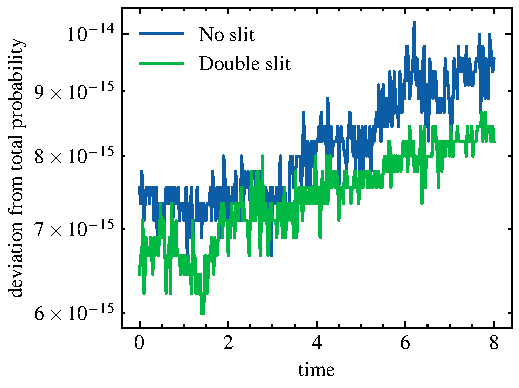
\includegraphics{results/problem_7/problem_7.pdf}
    \caption{Deviation from total probability as a function of time for both the absence (blue) and the presence (green) of a double slit. Mathematically, the figure displays \(1 - p(x,y;t)\), where \(p(x,y;t)\) is the probability density given in \eqref{eq:Born_rule}.}
    \label{fig:devation_from_probability}
\end{figure}


\subsection{Evolution of wave function}
\begin{figure*}[h!]
    \centering

    \subfloat[]{%
        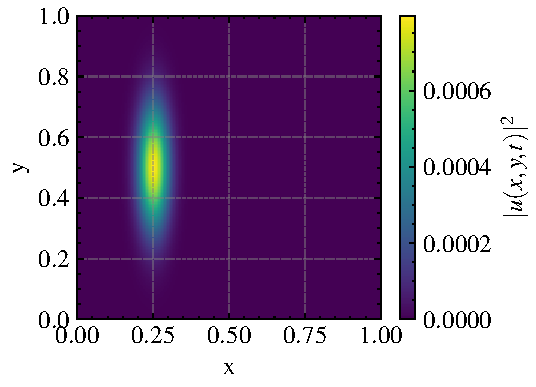
\includegraphics[width=0.33\linewidth]{results/problem_8/absolute_value0.pdf}%
    }\hfill
    \subfloat[]{%
        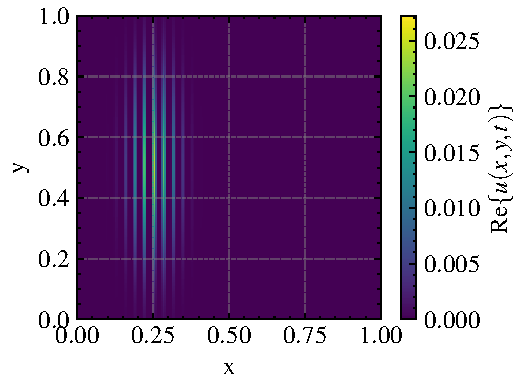
\includegraphics[width=0.33\linewidth]{results/problem_8/real_value0.pdf}%
    }\hfill
    \subfloat[]{%
        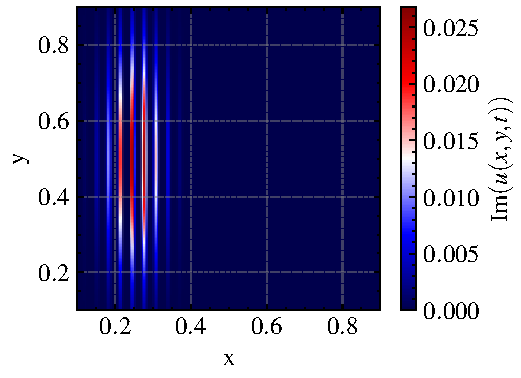
\includegraphics[width=0.33\linewidth]{results/problem_8/imag_value0.pdf}%
    }

    \caption{The absolute value squared (a), as well as the real (b) and imaginary (c) value, of the wave function at \(t=0 \ \si{ms}\).}
    \label{fig:evolution_wave_func}
\end{figure*}

\begin{figure*}[h!]
    \centering

    \subfloat[]{%
        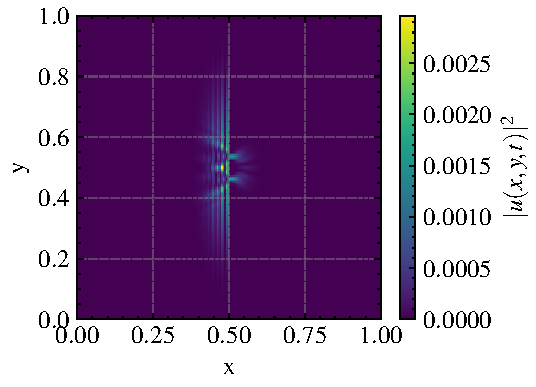
\includegraphics[width=0.33\linewidth]{results/problem_8/absolute_value0.001.pdf}%
    }\hfill
    \subfloat[]{%
        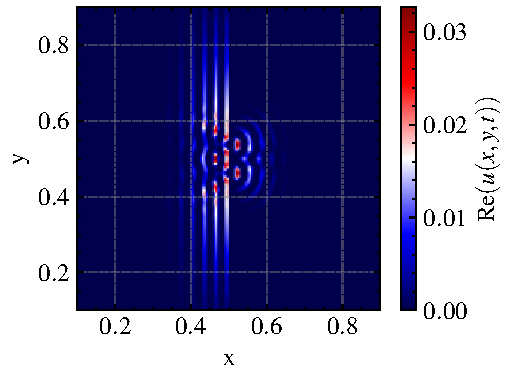
\includegraphics[width=0.33\linewidth]{results/problem_8/real_value0.001.pdf}%
    }\hfill
    \subfloat[]{%
        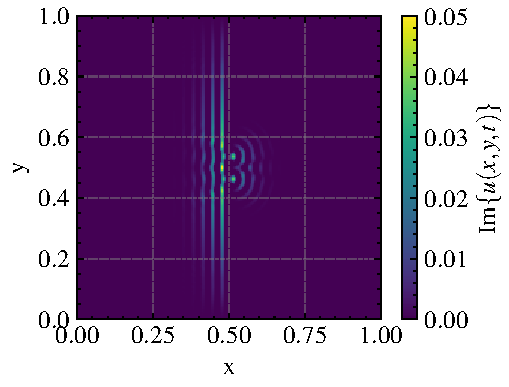
\includegraphics[width=0.33\linewidth]{results/problem_8/imag_value0.001.pdf}%
    }

    \caption{The absolute value squared (a), as well as the real (b) and imaginary (c) value, of the wave function at \(t=1 \ \si{ms}\).}
    \label{fig:evolution_wave_func}
\end{figure*}

\begin{figure*}[h!]
    \centering

    \subfloat[]{%
        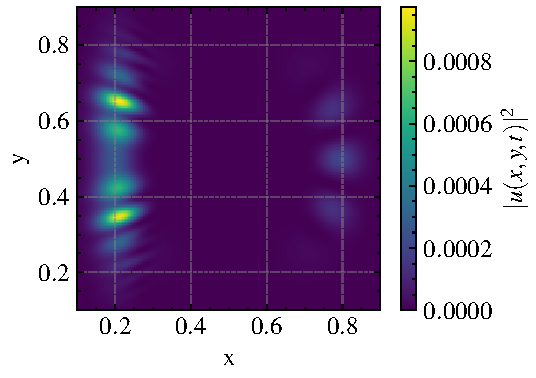
\includegraphics[width=0.33\linewidth]{results/problem_8/absolute_value0.002.pdf}%
    }\hfill
    \subfloat[]{%
        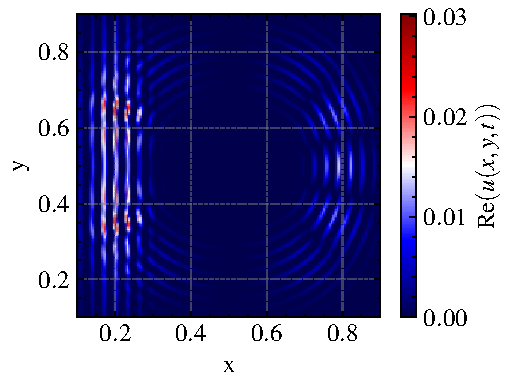
\includegraphics[width=0.33\linewidth]{results/problem_8/real_value0.002.pdf}%
    }\hfill
    \subfloat[]{%
        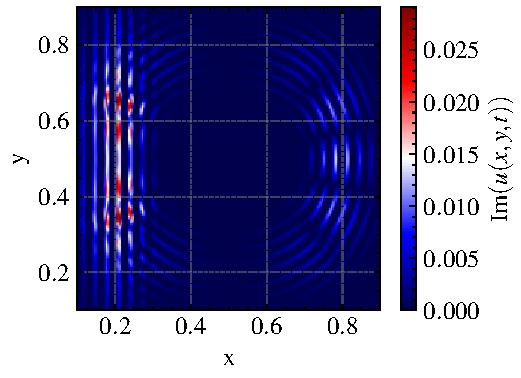
\includegraphics[width=0.33\linewidth]{results/problem_8/imag_value0.002.pdf}%
    }

    \caption{The absolute value squared (a), as well as the real (b) and imaginary (c) value, of the wave function at \(t=2 \ \si{ms}\).}
    \label{fig:evolution_wave_func}
\end{figure*}

\subsection{Interference pattern}
\begin{figure*}[h!]
    \centering

    \subfloat[]{%
        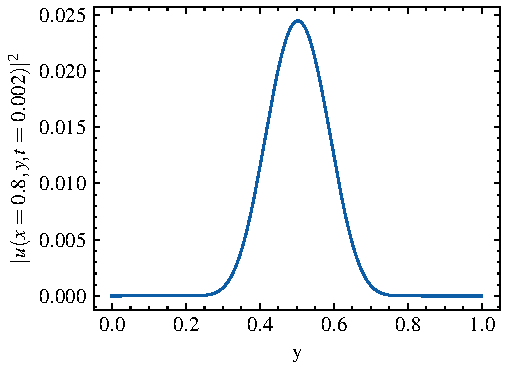
\includegraphics[width=0.33\linewidth]{results/problem_9/probability_x0p8_single.pdf}%
    }\hfill
    \subfloat[]{%
        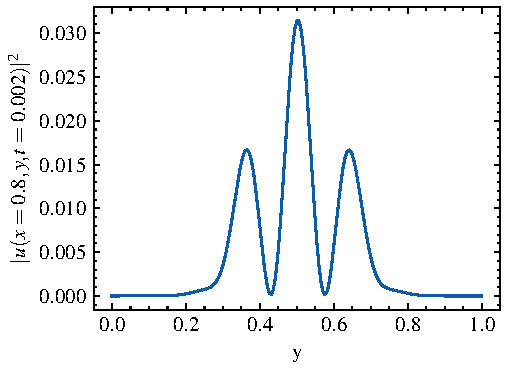
\includegraphics[width=0.33\linewidth]{results/problem_9/probability_x0p8_double.pdf}%
    }\hfill
    \subfloat[]{%
        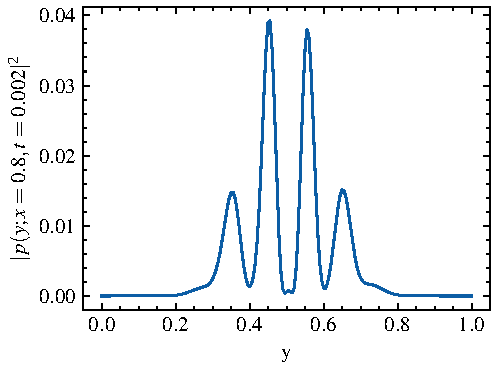
\includegraphics[width=0.33\linewidth]{results/problem_9/probability_x0p8_triple.pdf}%
    }
    \caption{The probability of detecting a particle along the \(y\)-axis, assuming a detection takes place at \(x=0.8\). The case of a single, double and triple slit are displayed in (a), (b) and (c), respectively.}
    \label{fig:probability_x0p8}
\end{figure*}



\section{Discussion}    \label{sec:discussion}

\section{Conclusion}

\newpage
\clearpage
\onecolumngrid
\appendix
\section{Appendix} \label{sec:code_excerpts}

\newpage

% \bibliographystyle{apalike}
% \bibliographystyle{unsrt}
\bibliographystyle{apsrev4-2}
\bibliography{references}


\end{document}
